\documentclass[11pt,journal,compsoc]{IEEEtran}

\usepackage[utf8]{inputenc}
\usepackage{xcolor}
\newcommand\todo[1]{\textcolor{red}{[#1]}}

\usepackage{tikz}
\usetikzlibrary{shapes,arrows}

\renewcommand\appendix{\par
  \setcounter{section}{0}
  \setcounter{subsection}{0}
  \setcounter{figure}{0}
  \setcounter{table}{0}
  \renewcommand\thesection{Appendix \Alph{section}}
  \renewcommand\thefigure{\Alph{section}\arabic{figure}}
  \renewcommand\thetable{\Alph{section}\arabic{table}}
}

% *** CITATION PACKAGES ***
%
\ifCLASSOPTIONcompsoc
  % IEEE Computer Society needs nocompress option
  % requires cite.sty v4.0 or later (November 2003)
  % \usepackage[nocompress]{cite}
\else
  % normal IEEE
  % \usepackage{cite}
\fi

% Define block styles
\tikzstyle{initBlock} = [draw, draw, fill=blue!20, 
    text width=6.5em, text badly centered, node distance=3cm, inner sep=0pt, minimum width=7em, minimum height=5em]
\tikzstyle{block} = [rectangle, draw, fill=green!20, text centered,text width=5em, rounded corners, minimum height=4em]
\tikzstyle{largerblock} = [rectangle, draw, fill=green!20,text centered, rounded corners, minimum height=4em]    
\tikzstyle{line} = [draw, -latex']
\tikzstyle{cloud} = [draw, ellipse,fill=blue!20, node distance=3cm,
    minimum height=2em]


% *** GRAPHICS RELATED PACKAGES ***
%
\ifCLASSINFOpdf
  % \usepackage[pdftex]{graphicx}
  % declare the path(s) where your graphic files are
  % \graphicspath{{../pdf/}{../jpeg/}}
  % and their extensions so you won't have to specify these with
  % every instance of \includegraphics
  % \DeclareGraphicsExtensions{.pdf,.jpeg,.png}
\else
  % or other class option (dvipsone, dvipdf, if not using dvips). graphicx
  % will default to the driver specified in the system graphics.cfg if no
  % driver is specified.
  % \usepackage[dvips]{graphicx}
  % declare the path(s) where your graphic files are
  % \graphicspath{{../eps/}}
  % and their extensions so you won't have to specify these with
  % every instance of \includegraphics
  % \DeclareGraphicsExtensions{.eps}
\fi

% *** TITLE/SUBJECT/AUTHOR/KEYWORDS INFO BELOW!!           ***
\newcommand\MYhyperrefoptions{bookmarks=true,bookmarksnumbered=true,
pdfpagemode={UseOutlines},plainpages=false,pdfpagelabels=true,
colorlinks=true,linkcolor={black},citecolor={black},urlcolor={black},
pdftitle={Bare Demo of IEEEtran.cls for Computer Society Journals},%<!CHANGE!
pdfsubject={Typesetting},%<!CHANGE!
pdfauthor={Michael D. Shell},%<!CHANGE!
pdfkeywords={Computer Society, IEEEtran, journal, LaTeX, paper,
             template}}%<^!CHANGE!

% correct bad hyphenation here
\hyphenation{op-tical net-works semi-conduc-tor}


\begin{document}
%
% paper title
\title{Artificial Intelligence and Decision Systems: Assignment \#3 - Resolution-based Theorem Prover}


\author{D. Monteiro (70125),$^\dagger$\thanks{$^\dagger$ MSc. student of Aerospace Engineering, Instituto Superior Técnico, Lisbon, Portugal. Student Nr: $70125$}, R.F. Santos (69278)$^\ddagger$\thanks{$^\ddagger$ MSc. student of Aerospace Engineering, Instituto Superior Técnico, Lisbon, Portugal. Student Nr: $69278$}\\[.2 cm]
\textit{University of Lisbon, Lisbon, Portugal}}% <-this % stops a space
     
        
%\IEEEcompsocitemizethanks{\IEEEcompsocthanksitem D. Monteiro, Aerospace Engineering Student in Instituto Superior Técnico, Lisbon, Portugal. Number 70125.\protect\\
% note need leading \protect in front of \\ to get a newline within \thanks as
% \\ is fragile and will error, could use \hfil\break instead.
%E-mail: diogo\_monteiro\_1$@$hotmail.com

%\IEEEcompsocthanksitem R. Santos, Aerospace Engineering Student in Instituto Superior Técnico, Lisbon, Portugal. Number 69278.\protect\\
% note need leading \protect in front of \\ to get a newline within \thanks as
% \\ is fragile and will error, could use \hfil\break instead.
%E-mail: rafael.j.f.santos$@$tecnico.ulisboa.pt}}

% note the % following the last \IEEEmembership and also \thanks - 
% these prevent an unwanted space from occurring between the last author name
% and the end of the author line. i.e., if you had this:
% 
% \author{....lastname \thanks{...} \thanks{...} }
%                     ^------------^------------^----Do not want these spaces!
%
% a space would be appended to the last name and could cause every name on that
% line to be shifted left slightly. This is one of those "LaTeX things". For
% instance, "\textbf{A} \textbf{B}" will typeset as "A B" not "AB". To get
% "AB" then you have to do: "\textbf{A}\textbf{B}"
% \thanks is no different in this regard, so shield the last } of each \thanks
% that ends a line with a % and do not let a space in before the next \thanks.
% Spaces after \IEEEmembership other than the last one are OK (and needed) as
% you are supposed to have spaces between the names. For what it is worth,
% this is a minor point as most people would not even notice if the said evil
% space somehow managed to creep in.



% The paper headers
%\markboth{Journal of \LaTeX\ Class Files,~Vol.~11, No.~4, December~2012}%
%{Shell \MakeLowercase{\textit{et al.}}: Bare Advanced Demo of IEEEtran.cls for Journals}

%\markboth{wadaw}%
%Shell \MakeLowercase{\textit{et al.}}: Artificial Intelligence and Decision Systems}


% The only time the second header will appear is for the odd numbered pages
% after the title page when using the twoside option.
% 
% *** Note that you probably will NOT want to include the author's ***
% *** name in the headers of peer review papers.                   ***
% You can use \ifCLASSOPTIONpeerreview for conditional compilation here if
% you desire.



% The publisher's ID mark at the bottom of the page is less important with
% Computer Society journal papers as those publications place the marks
% outside of the main text columns and, therefore, unlike regular IEEE
% journals, the available text space is not reduced by their presence.
% If you want to put a publisher's ID mark on the page you can do it like
% this:
%\IEEEpubid{0000--0000/00\$00.00~\copyright~2012 IEEE}
% or like this to get the Computer Society new two part style.
%\IEEEpubid{\makebox[\columnwidth]{\hfill 0000--0000/00/\$00.00~\copyright~2012 IEEE}%
%\hspace{\columnsep}\makebox[\columnwidth]{Published by the IEEE Computer Society\hfill}}
% Remember, if you use this you must call \IEEEpubidadjcol in the second
% column for its text to clear the IEEEpubid mark (Computer Society journal
% papers don't need this extra clearance.)



% use for special paper notices
%\IEEEspecialpapernotice{(Invited Paper)}



% for Computer Society papers, we must declare the abstract and index terms
% PRIOR to the title within the \IEEEtitleabstractindextext IEEEtran
% command as these need to go into the title area created by \maketitle.
% As a general rule, do not put math, special symbols or citations
% in the abstract or keywords.
\IEEEtitleabstractindextext{%
\begin{abstract}
In this assignment, a program was made in python to prove propositional logic theorems based on the resolution principle.
\end{abstract}

% Note that keywords are not normally used for peerreview papers.
\begin{IEEEkeywords}
resolution theorem, propositional logic, clausal normal form, CNF, knowledge base.
\end{IEEEkeywords}}


% make the title area
\maketitle

%\IEEEdisplaynontitleabstractindextext
% \IEEEdisplaynontitleabstractindextext has no effect when using
% compsoc under a non-conference mode.


% For peer review papers, you can put extra information on the cover
% page as needed:
% \ifCLASSOPTIONpeerreview
% \begin{center} \bfseries EDICS Category: 3-BBND \end{center}
% \fi
%
% For peerreview papers, this IEEEtran command inserts a page break and
% creates the second title. It will be ignored for other modes.
\IEEEpeerreviewmaketitle



\section{Introduction}

\IEEEPARstart{T}{he} aim of the present short report is to ...

\hfill 
 
\hfill \today

\section{Resolution Theorem Prover}




\section{Complementary Remarks}




% references section

% can use a bibliography generated by BibTeX as a .bbl file
% BibTeX documentation can be easily obtained at:
% http://www.ctan.org/tex-archive/biblio/bibtex/contrib/doc/
% The IEEEtran BibTeX style support page is at:
% http://www.michaelshell.org/tex/ieeetran/bibtex/
%\bibliographystyle{IEEEtran}
% argument is your BibTeX string definitions and bibliography database(s)
%\bibliography{IEEEabrv,../bib/paper}
%
% <OR> manually copy in the resultant .bbl file
% set second argument of \begin to the number of references
% (used to reserve space for the reference number labels box)
\begin{thebibliography}{1}

\bibitem{book}
S.~Russell and P.~Norvig, \emph{Atificial Intelligence - A Modern Approach}, 3rd~ed.\hskip 1em plus
  0.5em minus 0.4em\relax Pearson, 2010.

\end{thebibliography}

%\newpage
\onecolumn

%%%%%%%%%%%%%%%%%%%%%%

%% APPENDIX

%%%%%%%%%%%%%%%%%%%%%
\appendix
\section{Resolution Theorem Prover Algorithm} \label{app:resolutionloop}
\vfill
\begin{figure}[h]
\centering
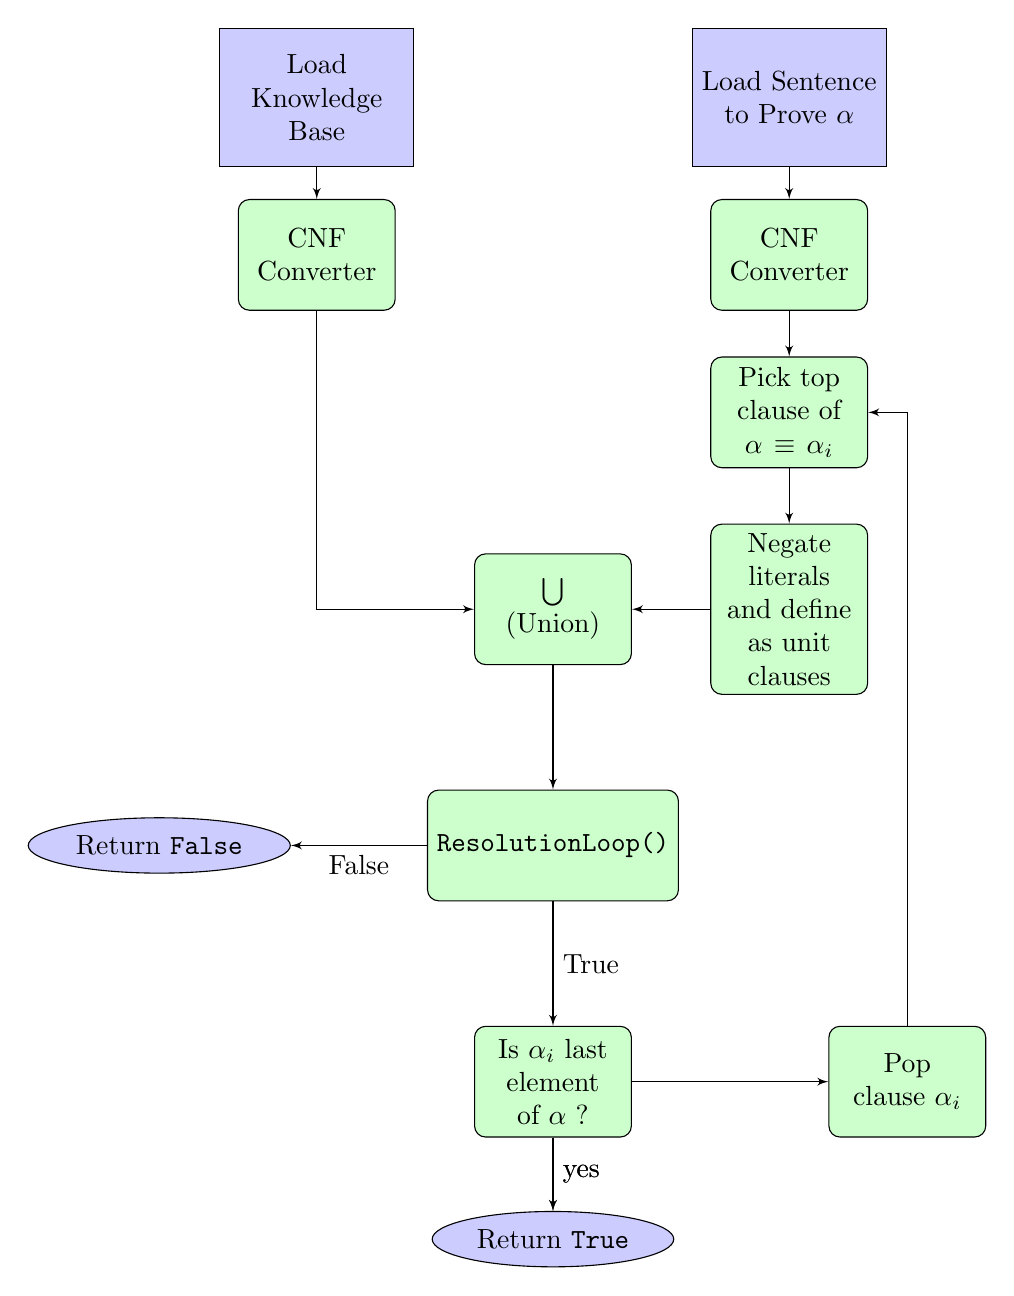
\begin{tikzpicture}[node distance = 2cm, auto]
    % Place nodes
    \node [initBlock] (kb) {Load Knowledge Base};
    \node [initBlock, right of=kb,node distance =6cm] (st) {Load Sentence to Prove $\alpha$};
    \node [block, below of=kb] (CNF1) {CNF Converter};
    \node [block, below of=st] (CNF2) {CNF Converter};
    \node [block, below of=CNF2] (pickClause) {Pick top clause of $\alpha \equiv\alpha_i$};
    \node [block, below of=pickClause,node distance=2.5cm] (negateLiterals) {Negate literals and define as unit clauses};
    \node [block, left of=negateLiterals,node distance=3cm] (union) {$\bigcup$\\(Union)};
    \node [largerblock, below of=union,node distance=3cm] (resolution) {\texttt{ResolutionLoop()}};
    \node [cloud, left of=resolution,node distance=5cm] (returnFalse) {Return \texttt{\textbf{False}}};
    \node [block, below of=resolution,node distance=3cm] (lastElement) {Is $\alpha_i$ last element of $\alpha$ ?};
    \node [block, right of=lastElement,node distance=4.5cm] (pop) {Pop clause $\alpha_i$};
    \node [cloud, below of=lastElement,node distance=2cm] (returnTrue) {Return \texttt{\textbf{True}}};
    %\node [cloud, right of=sentatomic, node distance=6cm] (return) {return};
 
	
    % Draw edges
    \path [line] (kb) -- (CNF1);
    \path [line] (CNF1) |- (union);
    \path [line] (union) -- (resolution);
    \path [line] (resolution) -- node {False} (returnFalse);
	\path [line] (resolution) -- node {True} (lastElement);
	\path [line] (lastElement) -- (pop);
	\path [line] (lastElement) -- node {yes} (returnTrue);
	\path [line] (lastElement) -- node {yes} (returnTrue);
	\path [line] (pop) |- (pickClause);    
    \path [line] (st) -- (CNF2);
     \path [line] (CNF2) -- (pickClause);
     \path [line] (pickClause) -- (negateLiterals);
    \path [line] (negateLiterals) -- (union);
	%\path [line] (sent2) -- node {no} (recursive2);    
	%\path [line] (recursive2) -- (operations);    
    %\path [line] (sent1) -- node {yes} (sent2);
    %\path [line] (sent2) -- node {yes} (operations);
    %\path [line] (operations) -| (return);
\end{tikzpicture}
\end{figure}
\vfill  
\newpage


\section{Move 'not' inwards flow chart} \label{app:moveNotInwards}
\vfill
\begin{figure}[h]
\centering
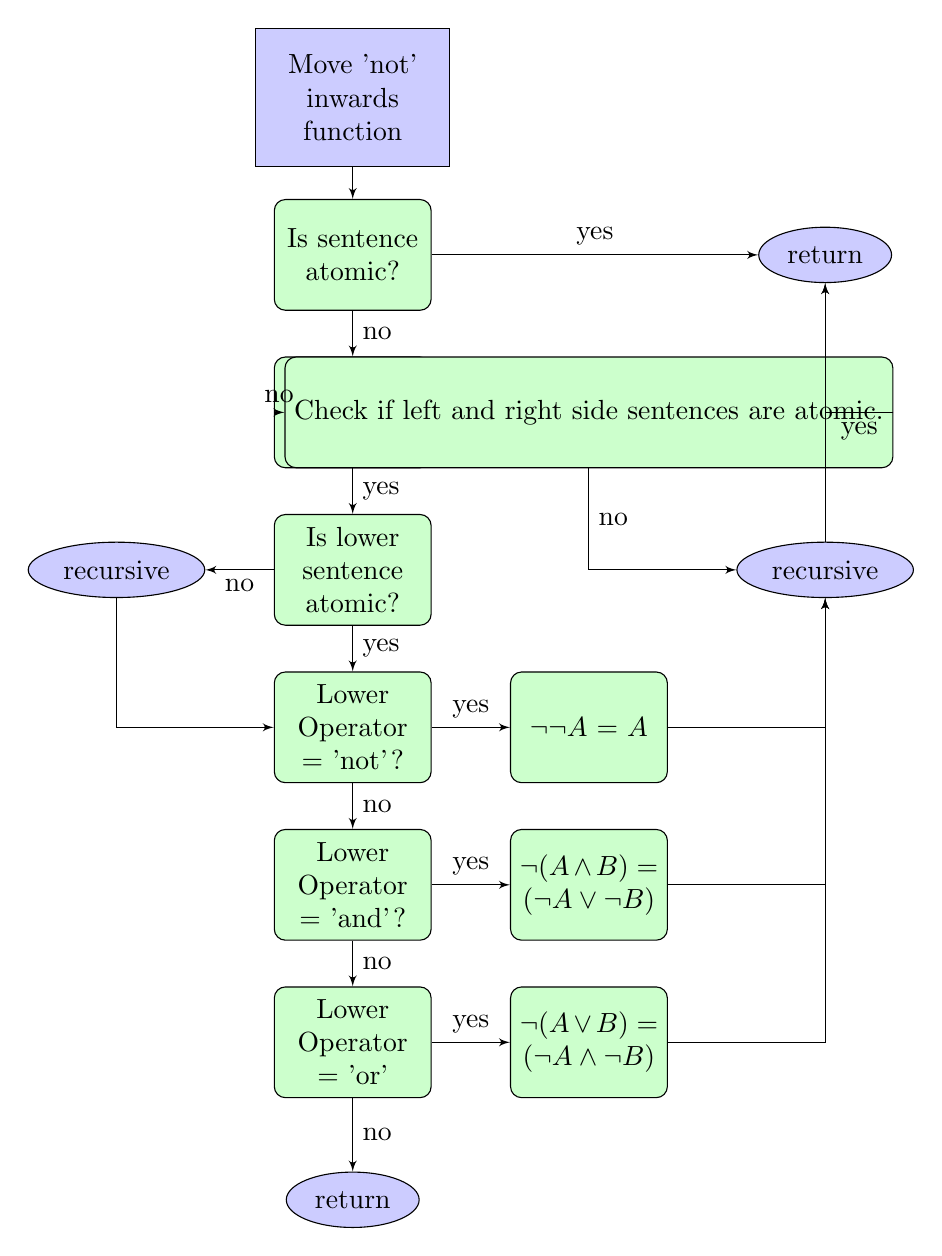
\begin{tikzpicture}[node distance = 2cm, auto]
    % Place nodes
    \node [initBlock] (init) {Move 'not' inwards function};
    \node [block, below of=init] (sentatomic) {Is sentence atomic?};
    \node [cloud, right of=sentatomic, node distance=6cm] (return) {return};
    \node [block, below of=sentatomic] (opnot) {Operator = 'not'?};
    \node [block, below of=opnot] (lowSent) {Is lower sentence atomic?};
    \node [block, below of=lowSent] (lowOpNot) {Lower Operator = 'not'?};
	\node [block, below of=lowOpNot] (lowOpAnd) {Lower Operator = 'and'?};
	\node [block, below of=lowOpAnd] (lowOpOr) {Lower Operator = 'or'};
    \node [block, right of=lowOpNot, node distance=3cm] (notnotA) {$\neg\neg A = A$};
	\node [block, right of=lowOpAnd, node distance=3cm] (morgan1) {$\neg (A \wedge B) = (\neg A \vee \neg B)$};
	\node [block, right of=lowOpOr, node distance=3cm] (morgan2) {$\neg (A \vee B) = (\neg A \wedge \neg B)$};
	\node [largerblock, right of=opnot, node distance=3cm] (sents) {Check if left and right side sentences are atomic.};
	\node [cloud, right of=lowSent, node distance=6cm] (recursive) {recursive};
	\node [cloud, left of=lowSent, node distance=3cm] (recursive2) {recursive};
	\node [cloud, below of=lowOpOr, node distance = 2cm] (return2) {return};
	%\node [largerblock, below of=lowSent, node distance=2.5cm] (lowOpAndOperations) {Check lower operator and do necessary operations};

    % Draw edges
    \path [line] (init) -- (sentatomic);
    \path [line] (sentatomic) -- node {no} (opnot);
    \path [line] (sentatomic) -- node {yes} (return);
    \path [line] (opnot) -- node {yes} (lowSent);
    \path [line] (opnot) -- node {no} (sents);
    	\path [line] (sents) -| node [near start]{yes} (return);
    	\path [line] (sents) |- node [near start]{no} (recursive);
    \path [line] (lowSent) -- node {yes} (lowOpNot);
    \path [line] (lowSent) -- node {no} (recursive2);
    \path [line] (recursive2) |- (lowOpNot);
    %\path [line] (lowOpAndOperations) -|(recursive);
	\path [line] (lowOpNot) --  node {no} (lowOpAnd);
	\path [line] (lowOpAnd) --  node {no} (lowOpOr);
    \path [line] (lowOpNot) -- node {yes} (notnotA);
    \path [line] (lowOpAnd) -- node {yes} (morgan1);
    \path [line] (lowOpOr) -- node {yes} (morgan2);
    \path [line] (notnotA) -| (recursive);
	\path [line] (morgan1) -| (recursive);
	\path [line] (morgan2) -| (recursive);
	\path [line] (recursive) -- (return);
	\path [line] (lowOpOr) -- node {no} (return2);
\end{tikzpicture}
\end{figure}
\vfill
\newpage
\section{Distributivity Law Flow Chart} \label{app:distribute}
\vfill
\begin{figure}[h]
\centering
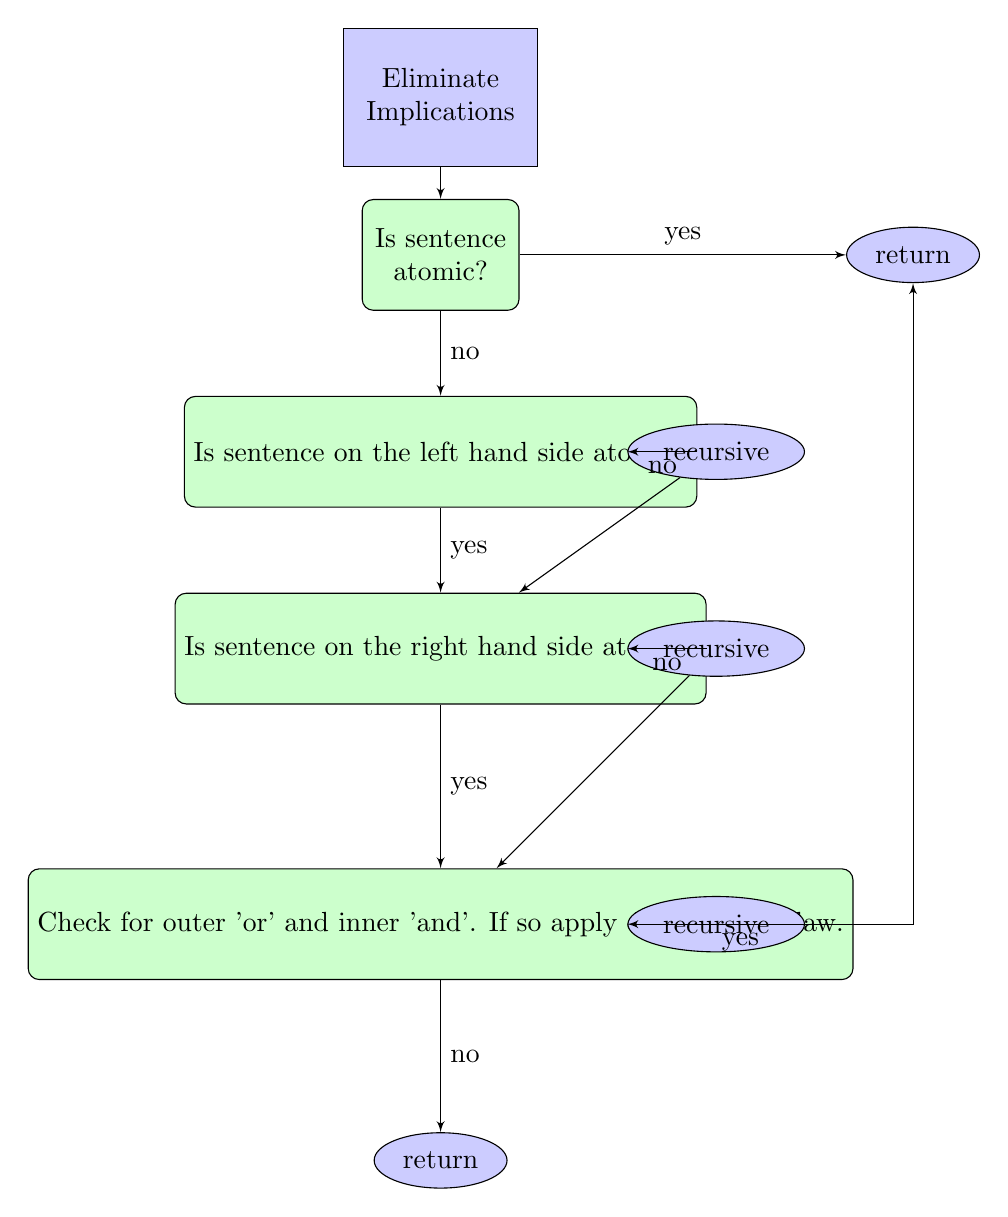
\begin{tikzpicture}[node distance = 2cm, auto]
    % Place nodes
    \node [initBlock] (init) {Eliminate Implications};
    \node [block, below of=init] (sentatomic) {Is sentence atomic?};
    \node [cloud, right of=sentatomic, node distance=6cm] (return) {return};
    %\node [block, below of=sentatomic, node distance = 3cm] (opnot) {Operator = 'not'?};
    \node [largerblock, below of=sentatomic, node distance = 2.5cm] (sent1) {Is sentence on the left hand side atomic?};
    %\node [largerblock, right of=opnot, node distance = 3.5cm] (sent1-2) {Is sentence on the left hand side atomic?};
    \node [largerblock, below of=sent1, node distance = 2.5cm] (sent2) {Is sentence on the right hand side atomic?};
	\node [largerblock, below of=sent2, node distance = 3.5cm] (operations) {Check for outer 'or' and inner 'and'. If so apply distributivity law.};
	\node [cloud, right of=sent1, node distance = 3.5cm] (recursive) {recursive};
	\node [cloud, right of=sent2, node distance = 3.5cm] (recursive2) {recursive};
	\node [cloud, right of=operations, node distance = 3.5cm] (recursive3) {recursive};
	\node [cloud, below of=operations, node distance = 3.0cm] (return2) {return};
    % Draw edges
    \path [line] (init) -- (sentatomic);
    %\path [line] (sentatomic) -- node {no} (opnot);
    \path [line] (sentatomic) -- node {yes} (return);
    \path [line] (sentatomic) -- node {no} (sent1);
	%\path [line] (opnot) -- node {yes} (sent1-2);
	%\path [line] (sent1-2) -- node {no} (recursive3);
	%\path [line] (sent1-2) -| node  [near start]{yes} (return);
	%\path [line] (recursive3) -- (return);    
    \path [line] (sent1) -- node {no} (recursive);
    \path [line] (recursive) -- (sent2);
	\path [line] (sent2) -- node {no} (recursive2);    
	\path [line] (recursive2) -- (operations);    
    \path [line] (sent1) -- node {yes} (sent2);
    \path [line] (sent2) -- node {yes} (operations);
    \path [line] (operations) -- node {yes} (recursive3);
    \path [line] (recursive3) -| (return);
    
    \path [line] (operations) -- node {no} (return2);
\end{tikzpicture}
\end{figure}
\vfill  
% biography section
% 
% If you have an EPS/PDF photo (graphicx package needed) extra braces are
% needed around the contents of the optional argument to biography to prevent
% the LaTeX parser from getting confused when it sees the complicated
% \includegraphics command within an optional argument. (You could create
% your own custom macro containing the \includegraphics command to make things
% simpler here.)
%\begin{IEEEbiography}[{\includegraphics[width=1in,height=1.25in,clip,keepaspectratio]{mshell}}]{Michael Shell}
% or if you just want to reserve a space for a photo:


\end{document}


